\usetikzlibrary{decorations.pathreplacing,decorations.pathmorphing,arrows.meta}

\begin{frame}{DNS resource records}
\begin{itemize}
\item resource record (RR) = single DNS database `entry'
\item has standard text and binary representation
    \begin{itemize}
    \item text used for server config files and display
    \item binary representation used for network protocol
    \end{itemize}
\end{itemize}
\end{frame}

\begin{frame}{DNS record example (text)}
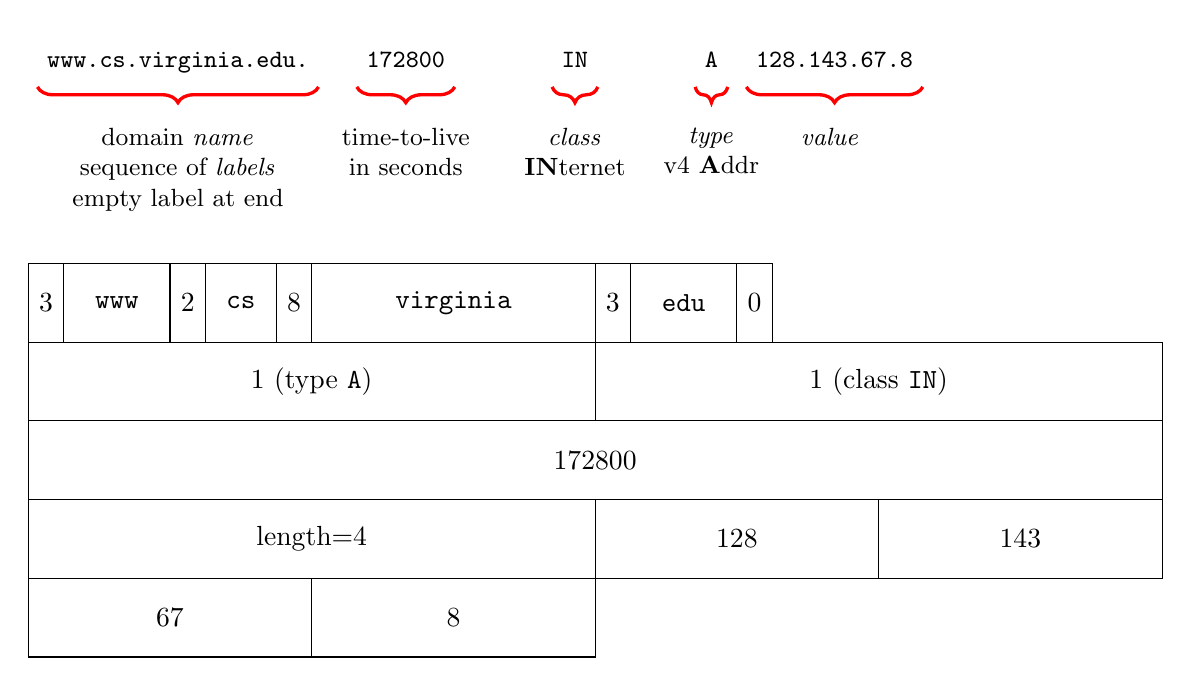
\begin{tikzpicture}
\matrix[ampersand replacement=\&,every node/.style={font=\small\tt\strut},column sep=0.5cm,anchor=north west] at (0,0) {
    \node (www) {www.cs.virginia.edu.}; \& \node (www ttl) {172800}; \&[.75cm]
    \node (www in) {IN}; \&[.75cm] \node (www a) {A}; \&[-.25cm]
    \node (www value) {128.143.67.8}; \\
};
\tikzset{
    mymark/.style={decorate,decoration={brace,amplitude=2mm},draw=red,very thick},
    mymark label/.style={draw=none,align=center,inner sep=5mm,font=\small},
}
\draw[mymark] (www.south east) -- (www.south west)
    node[below,midway,mymark label] {
        domain \textit{name} \\
        sequence of \textit{labels} \\
        empty label at end 
    };
\draw[mymark] (www ttl.south east) -- (www ttl.south west)
    node[below,midway,mymark label] {
        time-to-live \\
        in seconds
    };

\draw[mymark] (www in.south east) -- (www in.south west)
    node[below,midway,mymark label] {
        \textit{class} \\
        \textbf{IN}ternet
    };
\draw[mymark] (www a.south east) -- (www a.south west)
    node[below,midway,mymark label] {
        \textit{type} \\
        v4 \textbf{A}ddr
    };
\draw[mymark] (www value.south east) -- (www value.south west)
    node[below,midway,mymark label] {
        \textit{value}
    };
\begin{scope}[yshift=-3cm,x=0.45cm]
    \draw (0, 0) rectangle ++(1, -1) node[midway] {3};
    \draw (1, 0) rectangle ++(3, -1) node[midway] {\texttt{www}};
    \draw (4, 0) rectangle ++(1, -1) node[midway] {2};
    \draw (5, 0) rectangle ++(2, -1) node[midway] {\texttt{cs}};
    \draw (7, 0) rectangle ++(1, -1) node[midway] {8};
    \draw (8, 0) rectangle ++(8, -1) node[midway] {\texttt{virginia}};
    \draw (16, 0) rectangle ++(1, -1) node[midway] {3};
    \draw (17, 0) rectangle ++(3, -1) node[midway] {\texttt{edu}};
    \draw (20, 0) rectangle ++(1, -1) node[midway] {0};
    \draw (0, -1) rectangle ++(16, -1) node[midway] { 1 (type \texttt{A}) };
    \draw (16, -1) rectangle ++(16, -1) node[midway] { 1 (class \texttt{IN}) };
    \draw (0, -2) rectangle ++(32, -1) node[midway] {172800 };
    \draw (0, -3) rectangle ++(16, -1) node[midway] { length=4 };
    \draw (16, -3) rectangle ++(8, -1) node[midway] { 128 };
    \draw (24, -3) rectangle ++(8, -1) node[midway] { 143 };
    \draw (0, -4) rectangle ++(8, -1) node[midway] { 67 };
    \draw (8, -4) rectangle ++(8, -1) node[midway] { 8 };
\end{scope}
\end{tikzpicture}
\end{frame}

\begin{frame}{DNS name format}
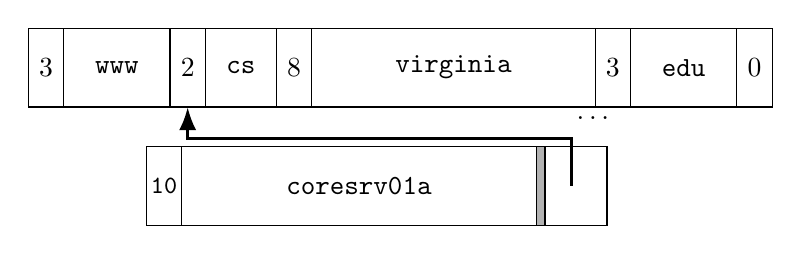
\begin{tikzpicture}
\begin{scope}[x=0.45cm]
    \draw (0, 0) rectangle ++(1, -1) node[midway] {3};
    \draw (1, 0) rectangle ++(3, -1) node[midway] {\texttt{www}};
    \coordinate (ptr end) at (4.5, -1);
    \draw (4, 0) rectangle ++(1, -1) node[midway] {2};
    \draw (5, 0) rectangle ++(2, -1) node[midway] {\texttt{cs}};
    \draw (7, 0) rectangle ++(1, -1) node[midway] {8};
    \draw (8, 0) rectangle ++(8, -1) node[midway] {\texttt{virginia}};
    \draw (16, 0) rectangle ++(1, -1) node[midway] {3};
    \draw (17, 0) rectangle ++(3, -1) node[midway] {\texttt{edu}};
    \draw (20, 0) rectangle ++(1, -1) node[midway] {0};
    \node[anchor=north] at (16, -1) {\ldots};
\end{scope}
\begin{scope}[x=0.45cm,yshift=-1.5cm,xshift=1.5cm]
    \draw (0, 0) rectangle ++(1, -1) node[midway,font=\small\tt] {10};
    \draw (1, 0) rectangle ++(10, -1) node[midway] {\texttt{coresrv01a}};
    \draw (11, 0) rectangle ++(2, -1);
    \draw[fill=black!30] (11, 0) rectangle ++ (0.25, -1);
    \coordinate (ptr base) at (12, -.5);
\end{scope}
\draw[very thick,-Latex] (ptr base) |- ([yshift=-.4cm]ptr end) -- (ptr end);
\end{tikzpicture}
\begin{itemize}
\item zero or more: length of $K>0$ followed by $K$ character case-insensitive \textit{label}
    \begin{itemize}
    \item labels limited to 64 bytes
    \end{itemize}
\item then either:
    \begin{itemize}
    \item length of $0$ to indicate end-of-name \textit{or}
    \item ``pointer'' to earlier name in message
        \begin{itemize}
        \item pointer encoded as \texttt{0xc000} + byte number in message (big endian)
        \item upper two bits being set prevents confusion with length
        \end{itemize}
    \end{itemize}
\end{itemize}
\end{frame}

